% Compile: xelatex usecase_standalone.tex
\documentclass[border=16pt]{standalone}
\usepackage{fontspec}
\usepackage{tikz}
\usetikzlibrary{shapes.geometric, fit, calc}

\definecolor{ensamBlue}{RGB}{0, 70, 127}
\definecolor{actorLine}{RGB}{70, 70, 70}
\definecolor{zoneFill}{RGB}{240, 246, 252}

\begin{document}
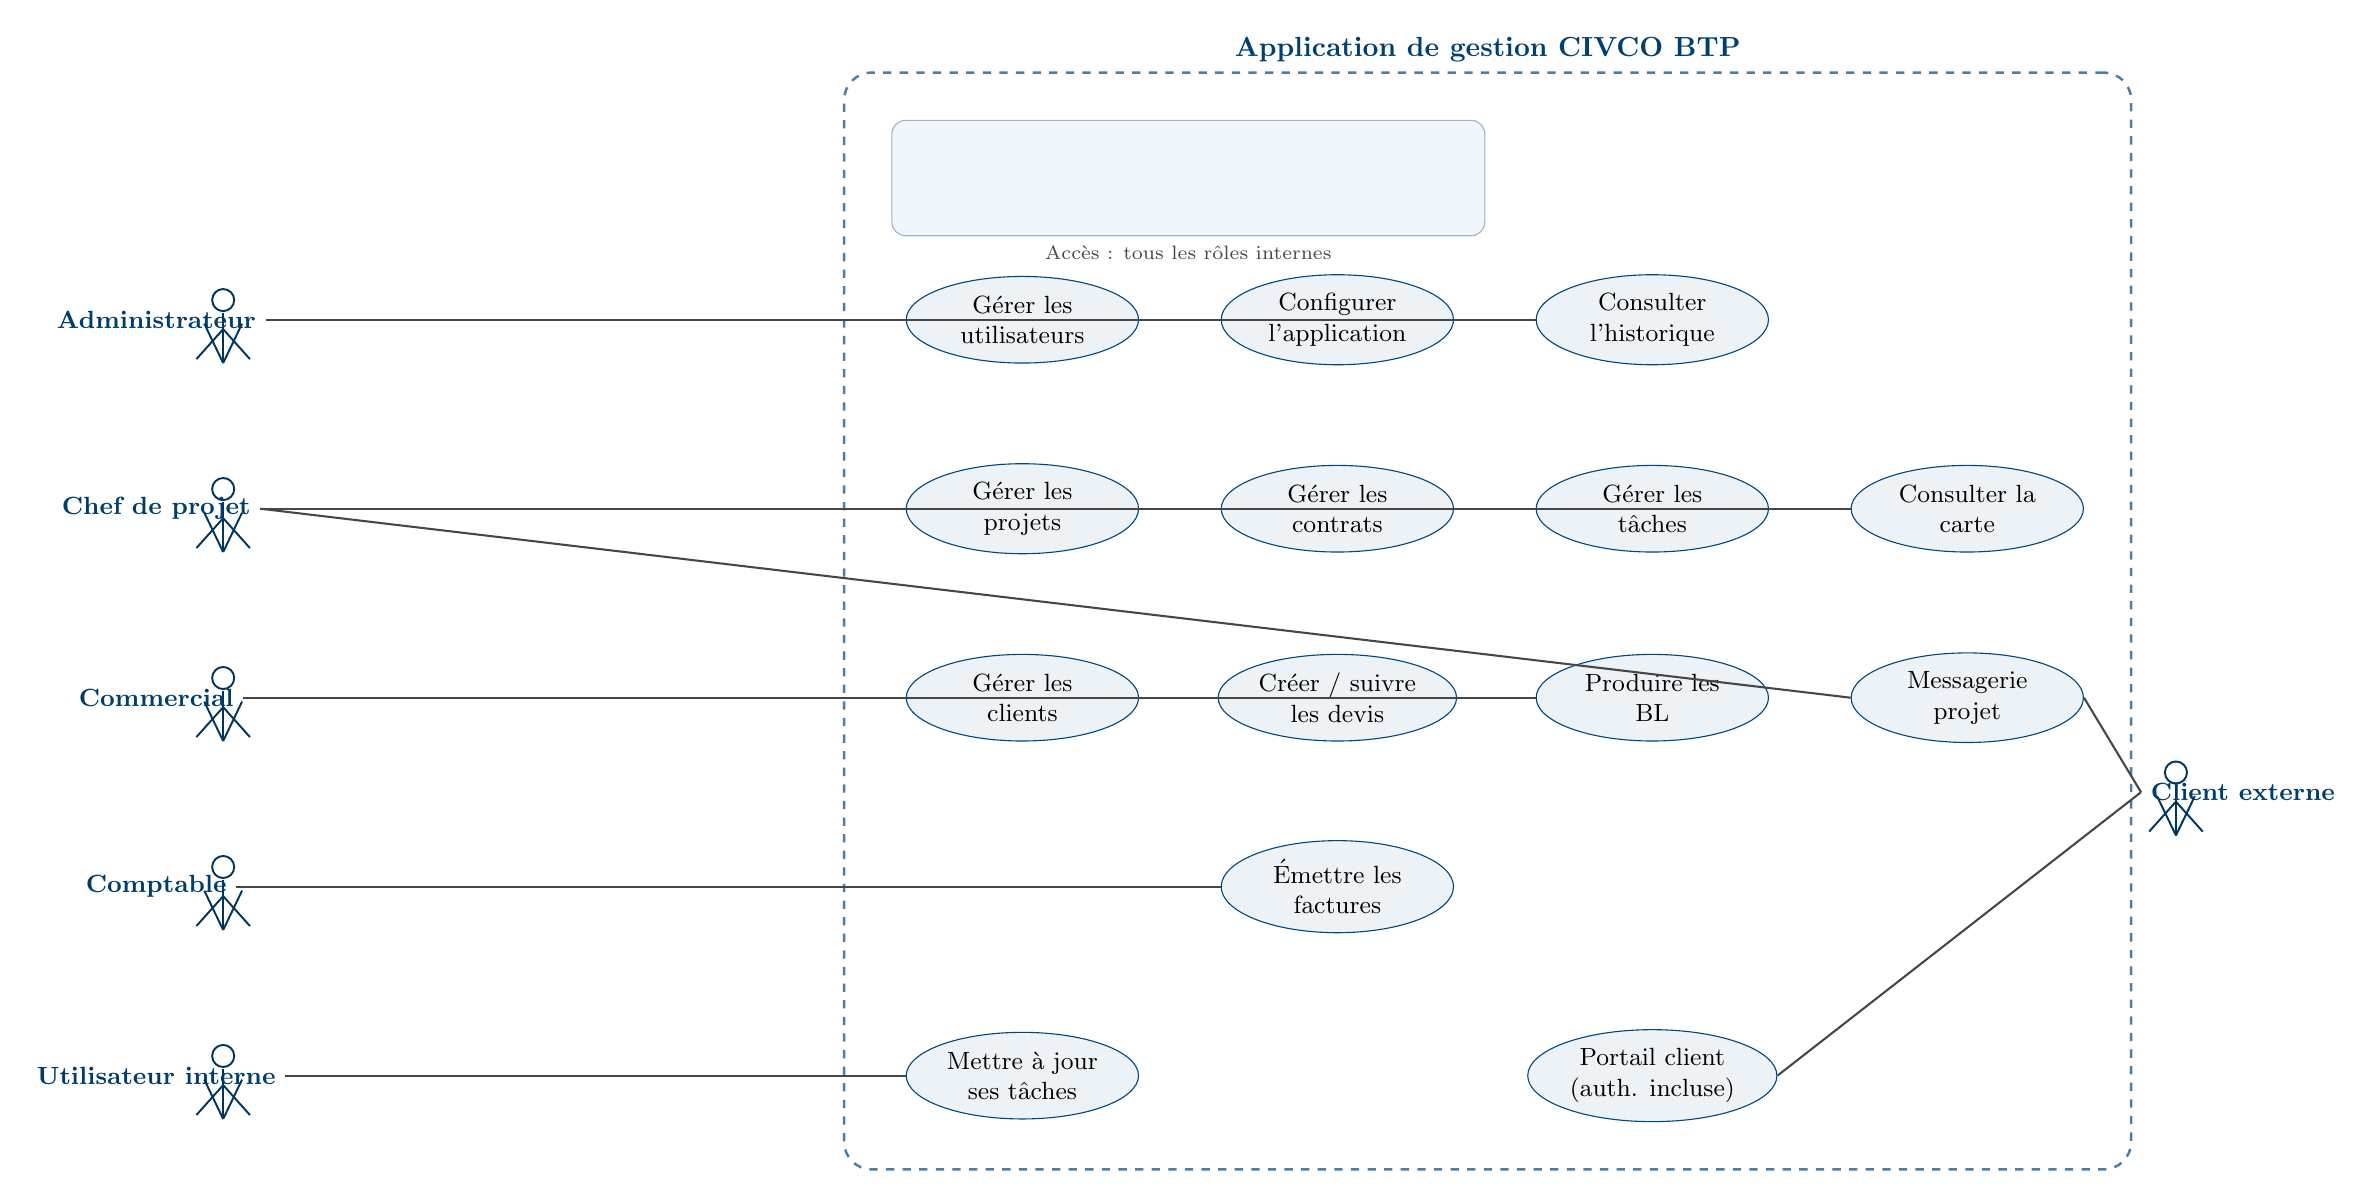
\begin{tikzpicture}[
  actor/.style={font=\small\bfseries, align=center, text=ensamBlue!85!black},
  uc/.style={
    ellipse,
    draw=ensamBlue,
    fill=ensamBlue!7,
    minimum width=2.95cm,
    minimum height=1.1cm,
    inner sep=2pt,
    align=center,
    font=\small
  },
  sys/.style={
    rectangle,
    draw=ensamBlue!70,
    dashed,
    line width=0.9pt,
    rounded corners=10pt
  },
  zone/.style={
    rectangle,
    draw=ensamBlue!40,
    fill=zoneFill,
    rounded corners=5pt,
    inner sep=5pt
  },
  assoc/.style={draw=actorLine, line width=0.75pt},
  stick/.style={draw=ensamBlue!75!black, line width=0.7pt}
]

  % ── Acteurs ────────────────────────────────────────────────────
  \node[actor] (admin)  at (-12.0,  4.8) {Administrateur};
  \node[actor] (pm)     at (-12.0,  2.4) {Chef de projet};
  \node[actor] (com)    at (-12.0,  0.0) {Commercial};
  \node[actor] (acc)    at (-12.0, -2.4) {Comptable};
  \node[actor] (user)   at (-12.0, -4.8) {Utilisateur interne};
  \node[actor] (client) at ( 14.5, -1.2) {Client externe};

  \foreach \X/\Y in {admin/4.8, pm/2.4, com/0.0, acc/-2.4, user/-4.8} {
    \draw[stick] (-11.15, \Y+0.25) circle (0.14);
    \draw[stick] (-11.15, \Y+0.08) -- (-11.15, \Y-0.55);
    \draw[stick] (-11.15, \Y-0.12) -- (-11.49, \Y-0.50);
    \draw[stick] (-11.15, \Y-0.12) -- (-10.81, \Y-0.50);
    \draw[stick] (-11.15, \Y-0.55) -- (-11.39, \Y-0.05);
    \draw[stick] (-11.15, \Y-0.55) -- (-10.91, \Y-0.05);
  }
  \draw[stick] (13.65, -0.95) circle (0.14);
  \draw[stick] (13.65, -1.12) -- (13.65, -1.75);
  \draw[stick] (13.65, -1.32) -- (13.31, -1.70);
  \draw[stick] (13.65, -1.32) -- (13.99, -1.70);
  \draw[stick] (13.65, -1.75) -- (13.41, -1.25);
  \draw[stick] (13.65, -1.75) -- (13.89, -1.25);

  % ── Cas d'utilisation (grille 4 × 6, sans chevauchement) ─────
  \node[uc] (uc1)  at (-1.0, 6.6) {S'authentifier};
  \node[uc] (uc2)  at ( 3.0, 6.6) {Consulter le\\tableau de bord};

  \node[uc] (uc3)  at (-1.0, 4.8) {Gérer les\\utilisateurs};
  \node[uc] (uc12) at ( 3.0, 4.8) {Configurer\\l'application};
  \node[uc] (uc13) at ( 7.0, 4.8) {Consulter\\l'historique};

  \node[uc] (uc4)  at (-1.0, 2.4) {Gérer les\\projets};
  \node[uc] (uc10) at ( 3.0, 2.4) {Gérer les\\contrats};
  \node[uc] (uc6)  at ( 7.0, 2.4) {Gérer les\\tâches};
  \node[uc] (uc11) at (11.0, 2.4) {Consulter la\\carte};

  \node[uc] (uc5)  at (-1.0, 0.0) {Gérer les\\clients};
  \node[uc] (uc7)  at ( 3.0, 0.0) {Créer / suivre\\les devis};
  \node[uc] (uc9)  at ( 7.0, 0.0) {Produire les\\BL};
  \node[uc] (uc14) at (11.0, 0.0) {Messagerie\\projet};

  \node[uc] (uc8)  at ( 3.0, -2.4) {Émettre les\\factures};

  \node[uc] (uc6b) at (-1.0, -4.8) {Mettre à jour\\ses tâches};
  \node[uc] (uc15) at ( 7.0, -4.8) {Portail client\\(auth. incluse)};

  \node[zone, fit=(uc1)(uc2),
        label={[font=\scriptsize, text=actorLine]below:{Accès : tous les rôles internes}}]
        (zoneCommon) {};

  \node[sys,
        fit=(zoneCommon)(uc3)(uc4)(uc5)(uc6)(uc6b)(uc7)(uc8)(uc9)(uc10)(uc11)(uc12)(uc13)(uc14)(uc15),
        inner sep=0.6cm,
        label={[font=\normalsize\bfseries, text=ensamBlue!90!black]above:%
          Application de gestion CIVCO BTP}
  ] (system) {};

  % ── Associations (depuis chaque acteur, une ligne par cas d'utilisation) ──
  \draw[assoc] (admin.east)  -- (uc3.west);
  \draw[assoc] (admin.east)  -- (uc12.west);
  \draw[assoc] (admin.east)  -- (uc13.west);

  \draw[assoc] (pm.east)     -- (uc4.west);
  \draw[assoc] (pm.east)     -- (uc10.west);
  \draw[assoc] (pm.east)     -- (uc6.west);
  \draw[assoc] (pm.east)     -- (uc11.west);
  \draw[assoc] (pm.east)     -- (uc14.west);

  \draw[assoc] (com.east)    -- (uc5.west);
  \draw[assoc] (com.east)    -- (uc7.west);
  \draw[assoc] (com.east)    -- (uc9.west);

  \draw[assoc] (acc.east)    -- (uc8.west);

  \draw[assoc] (user.east)   -- (uc6b.west);

  \draw[assoc] (client.west) -- (uc15.east);
  \draw[assoc] (client.west) -- (uc14.east);

\end{tikzpicture}
\end{document}
